\subsection{United States model (model ID: 08)}
The United States model (fig.~\ref{fig:08_schematic}) is part of a multi-model comparison study using several catchments in the United States \citep{Bai2009}. It has 2 stores and 5 parameters ($\alpha_{ei}$, $M$, $S_{max}$, $fc$, $\alpha_{ss}$). The model aims to represent:

\begin{itemizecompact}
\item Interception as a percentage of precipitation;
\item Separate unsaturated and saturated zones;
\item Separate bare soil evaporation and vegetation transpiration;
\item Saturation excess overland flow;
\item Subsurface flow.
\end{itemizecompact}

\subsubsection{File names}
\begin{tabular}{@{}ll}
Model: &m\_08\_us1\_5p\_2s \\
Parameter ranges: &m\_08\_us1\_5p\_2s\_parameter\_ ranges \\
\end{tabular}

% Equations
\subsubsection{Model equations}

% Model layout figure
{ 																	% This ensures it doesn't warp text further down
\begin{wrapfigure}{l}{5cm}
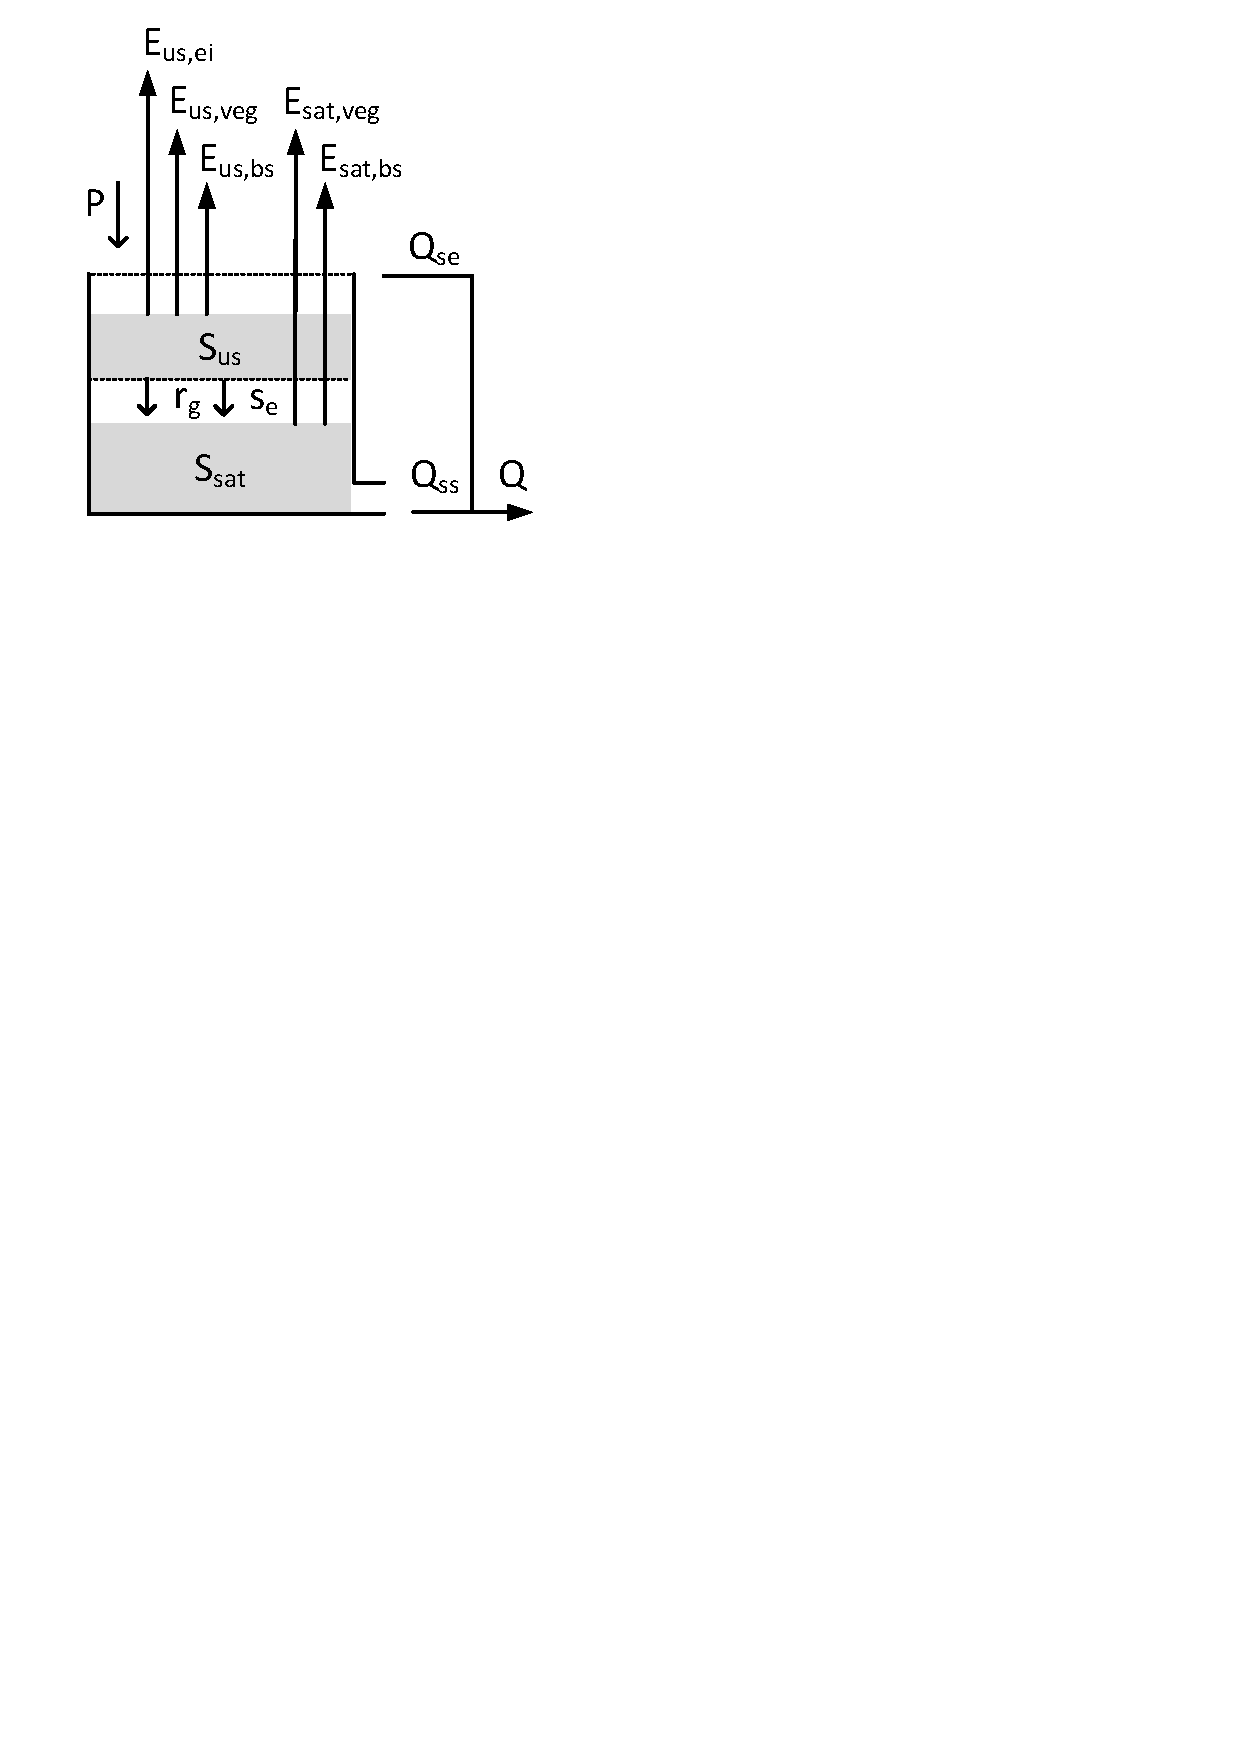
\includegraphics[trim=1cm 21cm 9cm 1cm,width=7cm,keepaspectratio]{./files/08_schematic.pdf}
\caption{Structure of the United States model} \label{fig:08_schematic}
\end{wrapfigure}

\begin{align}
	\frac{dS_{us}}{dt} &= P - E_{us,ei}-E_{us,veg}-E_{us,bs}-r_g \\
	E_{us,ei} &= \alpha_{ei}*P\\
	E_{us,veg} &= \begin{cases}
		\frac{S_{us}}{S_{us}+S_{sat}}*M*E_p, &\text{if } S_{us} > S_{usfc} \\
		\frac{S_{us}}{S_{us}+S_{sat}}*M*E_p*\frac{S_{us}}{S_{usfc}}, & \text{otherwise} \\
	\end{cases} \\
	E_{us,bs} &= \frac{S_{us}}{S_{us}+S_{sat}}*(1-M)*\frac{S_{us}}{S_{max}-S_{sat}}*E_p\\
	r_g &=\begin{cases}
		P, &\text{if } S_{us} > S_{usfc}\\
		0, & \text{otherwise} \\
	\end{cases}\\
	S_e &= \begin{cases}
			S_{us} - S_{usfc}, & if~S_{us} > S_{usfc}\\
			0, & \text{otherwise} \\
			\end{cases}\\
	S_{usfc} &= fc*(S_{max} - S_{sat})
\end{align}
} % end of wrap figure

Where $S_{us}$ [mm] is the current storage in the unsaturated zone, $E_{us,ei}$ $[mm/d]$ evaporation from interception, $E_{us,veg}$ $[mm/d]$ transpiration through vegetation, $E_{us,bs}$ $[mm/d]$ bare soil evaporation and $r_g$ $[mm/d]$ drainage to the saturated zone. Interception evaporation relies on parameter $\alpha_{ei}$ [-], representing the fraction of precipitation P that is intercepted. The implicit assumption is that this evaporates before the next precipitation event. Transpiration uses forest fraction $M$ [-], potential evapotranspiration $E_p$ $[mm/d]$ and the estimated field capacity $S_{usfc}$ through parameter $fc$ [-]. Bare soil evaporation relies also on the maximum soil moisture storage $S_{max}$ [mm]. 

\begin{align}
	\frac{dS_{sat}}{dt} &= r_g - E_{sat,veg}-E_{sat,bs} -Q_{se} - Q_{ss}\\
	E_{sat,veg} &= \frac{S_{sat}}{S_{max}}*M*E_p\\
	E_{sat,bs} &= \frac{S_{sat}}{S_{max}}*(1-M)*E_p\\
	Q_{se} &=\begin{cases}
		r_g, &\text{if } S_{us} \geq S_{max}\\
		0, & \text{otherwise} \\
	\end{cases}\\
	Q_{ss} &= \alpha_{ss}*S_{sat}
\end{align}

Where $S_{sat}$ [mm] is the current storage in the saturated zone, $E_{sat,veg}$ $[mm/d]$ transpiration through vegetation, $E_{sat,bs}$ $[mm/d]$ bare soil evaporation, $Q_{se}$ $[mm/d]$ saturation excess overland flow and $Q_{ss}$ $[mm/d]$ subsurface flow. Subsurface flow uses time parameter $\alpha_{ss}$ $[d^{-1}]$
Total flow:

\begin{align}
	Q &= Q_{se}+Q_{ss}
\end{align}

\subsubsection{Parameter overview}
% Table generated by Excel2LaTeX from sheet 'Sheet1'
\begin{table}[htbp]
  \centering
    \begin{tabular}{lll}
    \toprule
    Parameter & Unit  & Description \\
    \midrule
    $\alpha_{ei}$ & $-$   & Intercepted fraction of precipitation \\
    $M$   & $-$   & Forest fraction \\
    $S_{max}$ & $mm$  & Maximum soil moisture storage \\
    $fc$  & $-$   & Field capacity as fraction of $S_{max}$ \\
    $\alpha_{ss}$ & $d^{-1}$ & Runoff coefficient \\
    \bottomrule
    \end{tabular}%
  \label{tab:addlabel}%
\end{table}%

